\chapter{Speichertechnologien} %Zuerst
Nach den Ladesystemen werden in diesem Kapitel nun die Energiespeicher für Stadtbusse betrachtet. Wie im vorigen Kapitel werden zunächst die Bewertungskriterien und die betrachteten Technologien erläutert. In Tabelle \ref{vergleichstabelle_speichertechnologien} auf Seite \pageref{vergleichstabelle_speichertechnologien} werden die Werte aufgelistet.\\
Im Gegensatz zu den Ladesystemen ist die Produktvielfalt der Speichertechnologien nahezu unbegrenzt. Von daher werden hier keine konkreten Produkte verglichen, sondern es wurde versucht, die jeweils für den aktuellen Stand der Speichertechnologie relevanten Kenndaten zu finden.
\section{Bewertungskriterien} %TODO: Subsections
\section{Betrachtete Technologien}
Im folgenden Abschnitt werden die Grundlagen und die Einsatzgeschichten der verschiedenen Speichertechnologien kurz erläutert. Die Technologien sind nach dem genutzten physikalischen Effekt aufgeteilt \cite{Sterner:2014}[S. 35f]. Im realen Betrieb werden manchmal auch Kombinationen von verschiedenen Speichertechnologien eingesetzt, um dem hohen Leistungsbedarf beim Anfahren und bei der Bremsenergierückgewinnung gerecht zu werden.
\subsection{Mechanisch – Schwungradspeicher} %TODO: Quellen, warum endete die Gyrobuserprobung
In Bussen kann mechanische Energie mit einem Schwungrad gespeichert werden\footnote{Es gibt auch Prototypen von Pressluftspeichern in kleineren Fahrzeugen, in Bussen werden sie jedoch nur als Teil eines Hybridantriebs eingesetzt und hier nicht weiter betrachtet \cite{Sebastian-Naumann:2014}[S. 14].}, das die elektrische Energie in der Rotation des Schwungrades speichert. Die Energieübertragung erfolgt durch eine elektrische Motor- und Generatoreinheit. Moderne Schwungräder werden aus gewickelten Karbonfasern hergestellt und in Vakuumgehäusen magnetisch gelagert, sie erreichen hohe Drehzahlen und geringe Reibungsverluste \cite{993788}. Im Falle eines berstenden Schwungrades muss das Gehäuse die gesamte Energie innerhalb von Sekundenbruchteilen aufnehmen, ohne selbst zu bersten. Dies erfordert sehr schwere Gehäuse, die die spezifische Energie und Leistung eines tatsächlichen Systems stark reduzieren. Der Schwungradspeicher wurde in den fünfziger Jahren im Gyrobus im schweizerischen Yverdon auf einer acht Kilometer langen Linie erprobt. Die Strecke wurde erfolgreich zurückgelegt, die damalige Technologie war jedoch sehr wartungsaufwändig. Aktuell wird der Schwungradspeicher nur als Teil eines hybriden Antriebsstrangs eingesetzt.
\subsection{Elektrisch – Kondensator} %TODO: Quellen
Der Kondensator ist ein rein elektrischer Energiespeicher. Im klassischen Plattenkondensator werden zwei durch einen festes Dielektrikum getrennte Platten elektrisch aufgeladen, die Ladung kann später in Strom umgewandelt werden. Kondensatoren haben eine hohe spezifische Leistung, aber eine sehr geringe spezifische Energie. In Bussen werden sogenannte Superkondensatoren verwendet, die statt eines festen Dielektrikums ein Elektrolyt (meist eine Salz-Wasser-Lösung) verwenden. Die gelösten Ionen werden von der geladenen Platte angezogen, können sie jedoch aufgrund der umgebenden Ionenschicht nicht erreichen. Da der Abstand zwischen Platte un Ionen extrem klein ist, entsteht eine sehr hohe elektrische Kapazität. Eine weitere Kapazitätssteigerung wird durch die Einlagerung von einigen Elektronen des Elektrolyts in den Leiterplatten erreicht (siehe Abb. \ref{abb_doppelschicht}). \cite{Sterner:2014}[S. 167f]\\
\begin{figure}\centering
	 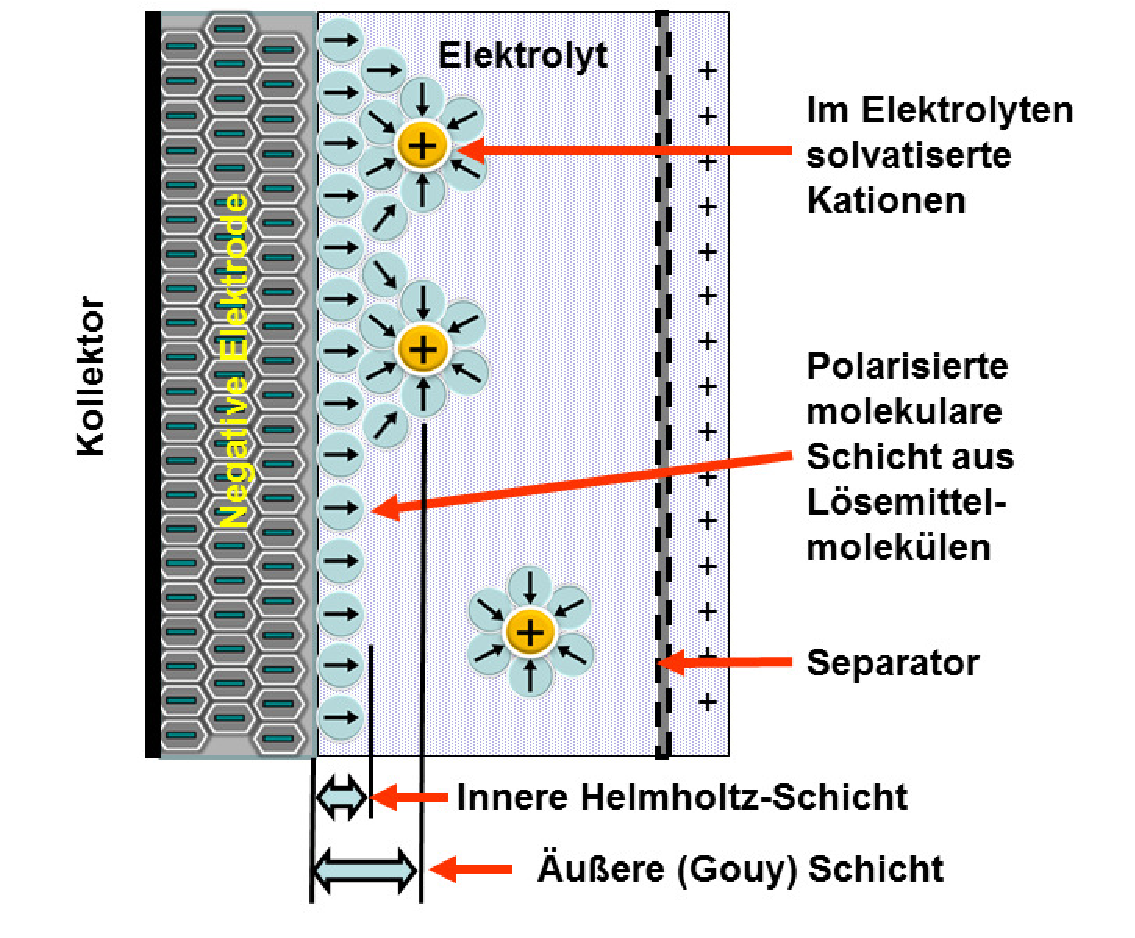
\includegraphics[width=0.5\textwidth]{Doppelschicht-Prinzipdarstellung}
	 \caption{Prinzipdarstellung der Doppelschichtkapazität. Quelle: Elcap (Own work) CC BY-SA 3.0, via Wikimedia Commons}
	 \label{abb_doppelschicht}
\end{figure}
In Shanghai werden Busse mit dieser Technologie seit 2008 im Linienverkehr eingesetzt, daneben werden Superkondensatoren für kurzzeitige Einsätze mit hohem Leistungsbedarf, zum Beispiel zur Bremsenergierückgewinnung oder zur Überbrückung stromloser Stellen in Trolleybussen eingesetzt \cite{Barminer-Busgesellschaft:2012}.
\subsection{Elektrochemisch – Batterie} %TODO: Besser
Batterien bestehen aus zwei Elektroden aus meist verschiedenen Metallen. Zwischen den Elektroden befindet sich ein Elektrolyt, in dem sich Ionen von der einen Elektrode zur anderen bewegen können. Durch die Bewegung der Ionen wird Ladung übertragen und an den Klemmen der Batterie entsteht eine Spannung. Batterien werden unterschieden in Primär- und Sekundärbatterien. Primärbatterien sind nicht wiederaufladbar und werden nicht weiter betrachtet \cite{KiehneBattery}[S. 1f].
\subsubsection{Blei-Säure}
Der Blei-Säure-Akkumulator besteht aus zwei Bleielektroden in einer Schwefelsäurelösung. Im entladenen Zustand bildet sich an beiden Elektronen Bleisulfat ($PbSO_4$). Die Elektrodengleichungen sind in Tabelle \ref{Pb} aufgeführt \cite{KiehneBattery}[S. 50].\\
\begin{table}
  \begin{tabularx}{\linewidth}{XrcX}
  	                   &                       $geladen$ & $\rightleftarrows$ & $entladen$            \\
  	Negative Elektrode & $PbO_2 + H_2SO_4 + 2H^+ + 2e^-$ & $\rightleftarrows$ & $PbSO_4 + 2H_2O$       \\
  	Positive Elektrode &                  $Pb + H_2SO_4$ & $\rightleftarrows$ & $PbSO_4 + 2H^+ + 2e^-$ \\ \midrule
  	Zellenreaktion     &         $Pb + PbO_2 + 2H_2SO_4$ & $\rightleftarrows$ & $2PbSO_4 + 2H_2O$
  \end{tabularx}
  \caption{Elektrodengleichungen der Blei-Säure-Batterie}
  \label{Pb}
\end{table}
Im Gegensatz zu den meisten anderen Batterien transportiert hier der Elektrolyt nicht nur die Ionen, sondern ist selbst an der Reaktion beteiligt.Im geladenen Zustand wird das enthaltene Wasser elektrolytisch zu Wasserstoff und Sauerstoff zerlegt. Dieser Wasserverlust muss durch periodisches nachfüllen oder Rekombination der Gase zu Wasser ausgeglichen werden. Vorteil der Gasentwicklung ist, das so durch Überladen die Spannungen verschiedener Zellen angeglichen werden können \cite{tub_aleph001746639}[S. 182].\\
Der Blei-Säure-Akkumulator ist eine der ältesten wiederaufladbaren Batterietechnologien und wurde in allen frühen Elektrobussen eingesetzt, zum Beispiel im weltweit ersten Batteriebus, der ab 1900 auf der Strecke Anhalter Bahnhof – Stettiner Bahnhof (heute: Nordbahnhof) in Berlin erprobt wurde \cite{Risch:1957}[S. 8f].

\subsubsection{Nickel-Cadmium} %TODO: Oder als Fußnote in NiMH?
Die Elektroden bestehen aus Nickelhydroxid und Cadmiumhydroxid in einem alkalischen, wässrigen Elektrolyt, dass nicht an der Reaktion beteiligt ist, sondern nur dem Ionentransport dient. Die Reaktionsgleichungen sind in Tabelle \ref{NiCd} aufgeführt\footnote{Dies ist eine vereinfachte Darstellung, der tatsächlich ablaufende Prozess ist noch nicht vollständig erforscht.} \cite{Sterner:2014}[S.233].\\
\begin{table}
  \begin{tabularx}{\linewidth}{XrcX}
  	                   &                       $geladen$ & $\rightleftarrows$ & $entladen$            \\
  	Negative Elektrode & $Cd + 2OH^-$ & $\rightleftarrows$ & $Cd(OH)_2 + 2e^-$       \\
  	Positive Elektrode &                  $2NiOOH + 2H_2O + 2e^-$ & $\rightleftarrows$ & $2Ni(OH)_2 + 2OH^-$ \\ \midrule
  	Zellenreaktion     &         $Cd + 2NiOOH + 2H_2O$ & $\rightleftarrows$ & $Cd(OH)_2 + 2Ni(OH)_2$
  \end{tabularx}
  \caption{Elektrodengleichungen der Nickel-Cadmium-Batterie}
  \label{NiCd}
\end{table}
Wie bei Blei-Säure-Batterien wird der Elektrolyt in Wasserstoff und Sauerstoff zerlegt, es sind offenen Bauformen und geschlossene Bauformen mit interner Rekombination vorhanden.\\
Die Nickel-Cadmium Batterie weist eine weit höhere spezifische Energie als die Blei-Säure-Batterie auf, wird jedoch in elektrischen Bussen nicht verwendet.

\subsubsection{Nickel-Metallhydrid}
Die Nickel-Mettalhydridbatterie verwendet wie die Nickel-Cadmiumbatterie eine Nickel(oxy)hydroxidelektrode und einen alkalischen Elektrolyt. Der Unterschied ist, das hier statt giftigem Cadmium(hydroxid) in der Negativen Elektrode Metall eingesetzt, in das $H^+$-Ionen zu Wasserstoff reduziert und eingelagert werden. Diese Hydrierung ist in mehreren Metallen möglich, in Batterien wird meist eine Mischung seltener Erden verwendet \cite{KiehneBattery}[S.85ff]. Die Reaktionsgleichungen sind in Tabelle \ref{NiMH} aufgeführt \cite{Sterner:2014}[S.245].\\
\begin{table}
  \begin{tabularx}{\linewidth}{XrcX}
  	                   &                       $geladen$ & $\rightleftarrows$ & $entladen$            \\
  	Negative Elektrode & $M(H) + OH^-$ & $\rightleftarrows$ & $M + H_2O + e^-$       \\
  	Positive Elektrode &                  $NiOOH + H_2O + e^-$ & $\rightleftarrows$ & $Ni(OH)_2 + OH^-$ \\ \midrule
  	Zellenreaktion     &         $M(H) + NiOOH + 2H_2O$ & $\rightleftarrows$ & $M + Ni(OH)_2$
  \end{tabularx}
  \caption{Elektrodengleichungen der Nickel-Metallhydrid-Batterie}
  \label{NiMH}
\end{table}
Der Nickel-Metallhydrid-Akku wird in mehreren Hybridfahrzeugen verwendet, zum Beispiel im Toyota Prius. Er weist eine hohe spezifische Energie, Leistung und Lebensdauer auf. Für die Verwendung als primärer Energiespeicher in Bussen ist die spezifische Energie jedoch immer noch zu niedrig.
\subsubsection{Lithium}
\subsubsection{Natrium-Schwefel} %TODO: Natrium-Nickelchlorid?
\subsubsection{Zink-Luft}
\section{Vergleichstabelle}   %TODO: AUSFÜLLEN!
\begin{table}[htbp]\centering
	\begin{tabularx}{\linewidth}{XXX}
		\toprule
		A1 & B1 & C1 \\ \midrule
		A2 & B2 & C2 \\
		A3 & B3 & C3 \\ \bottomrule
	\end{tabularx}
	\caption{Übersicht Ladesysteme}
	\label{vergleichstabelle_speichertechnologien}
\end{table}